\documentclass[11pt]{article}

% ---------------------------------------------------------------- packages ---
\usepackage[margin=1in]{geometry}
\usepackage{microtype}
\usepackage[T1]{fontenc}
\usepackage{lmodern}
\usepackage{amsmath}
\usepackage{xcolor}
\usepackage{enumitem}
\usepackage{booktabs}
\usepackage{titlesec}
\usepackage{tikz}
\usetikzlibrary{positioning,arrows.meta,shapes.geometric,backgrounds,fit,calc}
\usepackage[hidelinks]{hyperref}

% ------------------------------------------------------------------ palette ---
\definecolor{kailoink}{HTML}{16232B}
\definecolor{kailoaccent}{HTML}{0B6E77}
\definecolor{kailorule}{HTML}{C4CCD2}
\definecolor{kailosoft}{HTML}{E8EEF0}
\definecolor{kailowarn}{HTML}{A6521A}
\definecolor{kailogood}{HTML}{2F6D4F}
\definecolor{boxbg}{HTML}{F4F7F8}

\hypersetup{colorlinks=true,linkcolor=kailoaccent,urlcolor=kailoaccent}

% ---------------------------------------------------------------- headings ---
\titleformat{\section}{\Large\bfseries\color{kailoink}}{\thesection}{0.6em}{}
\titleformat{\subsection}{\large\bfseries\color{kailoink}}{\thesubsection}{0.6em}{}
\titleformat{\subsubsection}{\normalsize\bfseries\color{kailoaccent}}{}{0em}{}
\titlespacing*{\section}{0pt}{1.6em}{0.7em}

\setlist[itemize]{leftmargin=1.3em,itemsep=2pt,topsep=3pt}
\setlist[enumerate]{leftmargin=1.5em,itemsep=2pt,topsep=3pt}

% a light callout box
\newcommand{\assess}[1]{%
  \par\vspace{4pt}%
  \noindent\colorbox{boxbg}{\parbox{\dimexpr\linewidth-2\fboxsep}{%
  \small\textcolor{kailowarn}{\textbf{Assessment.}}\;#1}}\par\vspace{4pt}}

\newcommand{\code}[1]{\texttt{\small #1}}

% ================================================================== title ===
\begin{document}
\begin{center}
  {\LARGE\bfseries\color{kailoink} Kailo Coaching Hub Audit}\\[6pt]
  {\large\color{kailoaccent} Product review \& data-platform architecture}\\[10pt]
  {\normalsize 21 August 2026}
\end{center}
\vspace{0.5em}
\hrule height 1pt
\vspace{1.2em}

% --------------------------------------------------------------- framing ---
\section*{Defining Product Goals}
\addcontentsline{toc}{section}{Defining Product Goals}

\begin{itemize}
  \item \textbf{Team-native, coach-facing training platform.} The team is the
    unit; the coach is the primary user.
  \item \textbf{Stronger analytical tools and coach customization} than
    TrainingPeaks or FinalSurge --- the analytics and the ability to tailor the
    surface are the differentiators, not feature parity.
  \item \textbf{A coach-determined path for athletes to interact} that
    \emph{reduces} the need for athlete buy-in. The less work an athlete has to
    do, the better the product: participation should be near-passive by default,
    with the coach deciding how much the athlete is asked to do.
\end{itemize}

\subsection*{Technical Needs}
\begin{itemize}
  \item \textbf{Athlete objects with histories and attributes.} Each athlete
    carries a history (race and training paces over time) \emph{and} a set of
    learned attributes --- e.g.\ ``performs better on hilly courses,''
    ``degrades more in rain / heat.'' These attributes are estimated from data,
    they change as more data arrives, and the set will grow. The data platform
    exists to populate and keep refreshing them.
\end{itemize}

\vspace{0.4em}
\hrule height 0.4pt
\vspace{0.6em}

% ============================================================ 1. AUDIT ===
\section{Product Audit}

\subsection{Organization}

The current coaching hub (desktop) is organized on two axes: a \textbf{thematic
vertical axis} and a \textbf{temporal horizontal axis}. The vertical axis is a
left pane on wide screens, moving to the top on narrow screens. None of its
top-level labels are clickable. Its structure:

\begin{center}
\small
\begin{tabular}{@{}p{0.30\linewidth} p{0.30\linewidth} p{0.30\linewidth}@{}}
\toprule
\textbf{Before Practice} & \textbf{After Practice} & \textbf{The Roster}\\
\midrule
Today & Session review & Week wall\\
Tasks + Links & Inbox & Volume\\
\quad Planner & & Athlete\\
\quad Workout planner & & \quad Parameters\\
\quad Pace cards & & \quad Results\\
Share with the Team & & \quad Predictions\\
\quad Athlete day & & \\
\quad Team board & \textbf{Housekeeping} & \\
\quad 1-on-1s & Operations & \\
 & Data health & \\
 & How this works & \\
 & Setup & \\
\bottomrule
\end{tabular}
\end{center}

\subsubsection{The landing page (\code{kailo.fit/hub}, ``Today'')}
The landing page is a long stack of text widgets. Top widgets include
\emph{``[N] uploaded yesterday,'' ``Available today,'' ``Data flags,'' ``Gone
quiet,'' ``Need a look,''} and \emph{``Dew point at practice.''} Below these sit
more text widgets: \emph{``Where your attention goes''} (activities flagged as
abnormal --- average heart rate high on an easy run, distance longer than
expected), a \emph{``Today's plan''} widget with a print option, and a practice
conditions widget (\emph{``Conditions this afternoon''}).

Specific notes:
\begin{itemize}
  \item \textbf{Keep high-quality, accessible print.} The plan's print option is
    good and should stay easy to reach throughout.
  \item \textbf{Conditions is buried and single-window.} ``Conditions this
    afternoon'' sits too far down, does not currently populate, and only shows
    the afternoon --- athletes running \emph{doubles} lose the morning window
    entirely.
  \item \textbf{No expand/collapse} on any widget, producing a very long page.
\end{itemize}

\assess{There is too much information, almost all of it text, with no visual
hierarchy to separate what matters from what does not. Because this is the
landing page, deep customization is essential --- and this critique of the
landing page is the critique of the whole product.}

\subsection{Proposed structure: five main tabs}

Collapse the sprawl into five tabs.

\begin{enumerate}
  \item \textbf{Today} --- weather for \emph{four} windows: this morning, this
    afternoon, next morning, next afternoon (fixing the doubles gap).
  \item \textbf{Upcoming.}
  \item \textbf{Athletes} --- see the athlete-page layout below.
  \item \textbf{Recruiting.}
  \item \textbf{Settings.}
\end{enumerate}

\subsubsection{The athlete page (three tiers, top to bottom)}
\begin{description}[leftmargin=0em,style=nextline,itemsep=3pt]
  \item[Identity (top, glanceable).] Name, gender, class, hometown, MileSplit
    and Athletic.net links, and PRs.
  \item[Secondary.] Attendance / training log, past and current injuries,
    upcoming registered events (date, name, event), training paces.
  \item[Advanced analytics (bottom).] The learned attribute models:
    \begin{itemize}
      \item \textbf{Hill Resilience} --- is the runner better on flat or hilly
        courses? Built from course-elevation learning, MileSplit course
        rankings, FloRatings A/B/C/D, TullyRunners speed ratings, joshm.dev's
        Crystal Springs Pace Factor, and the golf-slope-rating analog.
      \item \textbf{Weather Impact} --- how much adverse weather degrades this
        runner. The constraint: exact per-race time is needed, and getting it at
        scale from Athletic.net is not viable (see \S\ref{sec:platform}).
      \item Additional analytical models as desired.
    \end{itemize}
\end{description}

\subsection{Wording}

Much of the copy reads as too cute, too artsy, or too AI-generated, and should
be plainer. Examples:

\begin{center}
\small
\begin{tabular}{@{}p{0.52\linewidth} p{0.42\linewidth}@{}}
\toprule
\textbf{Current} & \textbf{Plainer}\\
\midrule
``One line from an athlete at 3:47 is worth more than finding out at 4:10 in the
parking lot.'' & Cut, or state the actual point.\\[4pt]
``Where your attention goes'' --- ``ranked, and every name is a door.'' & ``Needs
a look,'' with names that link.\\[4pt]
``Yesterday, rolled up'' & ``Yesterday, summarized.''\\
\bottomrule
\end{tabular}
\end{center}

% ==================================================== 2. DATA PLATFORM ===
\section{Data and Enrichment Platform}
\label{sec:platform}

The athlete attributes in \S1 (hill resilience, weather impact, and the models
to come) are only as good as the data feeding them. This section lays out how
that data is sourced, enriched, and linked --- and why the platform must
\textbf{divest fully from Athletic.net} as a scale dependency.

% ------------------------------------------------------------ DIAGRAM 1 ---
\subsection{(1) Roster, meet, and team information}

\begin{figure}[h]
\centering
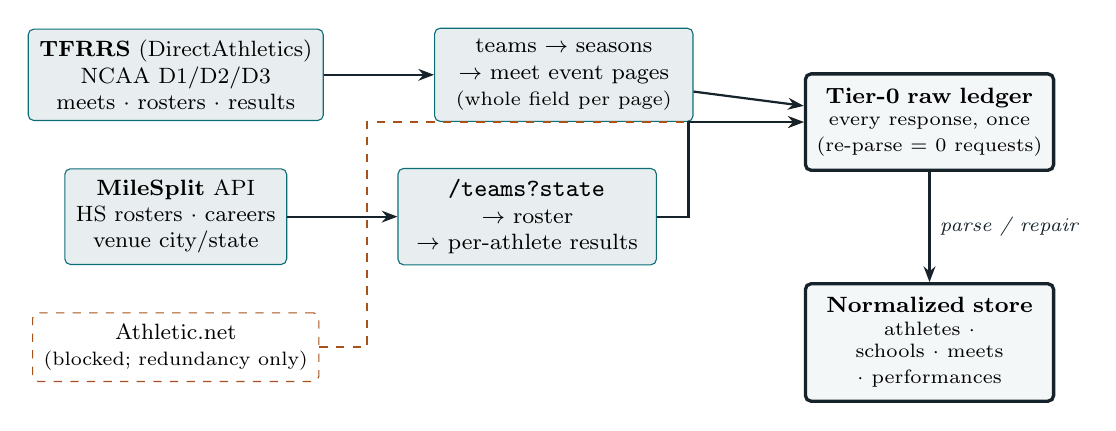
\begin{tikzpicture}[
  font=\footnotesize,
  node distance=6mm,
  src/.style={draw=kailoaccent,fill=kailosoft,rounded corners=2pt,
              minimum height=8mm,align=center,inner sep=4pt},
  dead/.style={draw=kailowarn,fill=white,rounded corners=2pt,
               minimum height=8mm,align=center,inner sep=4pt,dashed},
  store/.style={draw=kailoink,fill=boxbg,rounded corners=2pt,
                minimum height=9mm,align=center,inner sep=5pt,very thick},
  arr/.style={-{Stealth[length=2mm]},kailoink,thick},
  darr/.style={-{Stealth[length=2mm]},kailowarn,thick,dashed},
  lbl/.style={font=\scriptsize\itshape,text=kailoink}
]
% sources column
\node[src] (tfrrs) {\textbf{TFRRS} (DirectAthletics)\\ NCAA D1/D2/D3\\ meets $\cdot$ rosters $\cdot$ results};
\node[src,below=of tfrrs] (ms) {\textbf{MileSplit} API\\ HS rosters $\cdot$ careers\\ venue city/state};
\node[dead,below=of ms] (anet) {Athletic.net\\ \scriptsize(blocked; redundancy only)};

% method middle
\node[src,right=14mm of tfrrs,text width=30mm] (mtfrrs)
  {teams $\to$ seasons\\ $\to$ meet event pages\\
   \scriptsize(whole field per page)};
\node[src,right=14mm of ms,text width=30mm] (mms)
  {\code{/teams?state} $\to$ roster\\ $\to$ per-athlete results};

% ledger + store
\node[store,right=14mm of mtfrrs,yshift=-6mm,text width=28mm] (ledger)
  {\textbf{Tier-0 raw ledger}\\ \scriptsize every response, once\\
   \scriptsize(re-parse $=$ 0 requests)};
\node[store,below=14mm of ledger,text width=28mm] (db)
  {\textbf{Normalized store}\\ \scriptsize athletes $\cdot$ schools $\cdot$ meets\\
   \scriptsize $\cdot$ performances};

\draw[arr] (tfrrs) -- (mtfrrs);
\draw[arr] (ms) -- (mms);
\draw[darr] (anet.east) -- ++(6mm,0) |- (ledger.west);
\draw[arr] (mtfrrs) -- (ledger);
\draw[arr] (mms.east) -- ++(4mm,0) |- (ledger.west);
\draw[arr] (ledger) -- (db) node[lbl,midway,right] {parse / repair};
\end{tikzpicture}
\caption{Roster/meet/team sourcing. Every response tees to a raw ledger before
parsing, so a parser fix replays at zero request cost. Athletic.net (dashed)
is demoted to redundancy.}
\end{figure}

\noindent\textbf{How it works, per source.}
\begin{itemize}
  \item \textbf{TFRRS (college).} Seeded from the seven NCAA-division region
    pages, walk teams $\to$ seasons $\to$ meets. A single meet \emph{event} page
    carries the whole field (place, athlete, class year, team, mark), so one
    fetch covers every school in a race. Corpus: 8.1M rows, all three divisions,
    XC + indoor + outdoor, 2021--2026.
  \item \textbf{MileSplit (HS).} \code{/teams?state=xx} then the proven
    per-team, per-athlete ingest path, smallest state first. Polite by default
    (rate-limited, ledger tee). Note the enumeration cap: \code{/teams?state}
    returns at most 999 rows, so the largest states need a per-county or
    meet-harvest route for full coverage.
  \item \textbf{Divest path.} Athletic.net has the broadest US high-school
    coverage and the project was built on it, but it is not a dependency to
    scale on: Cloudflare returns \code{cf-mitigated=challenge} on sustained
    crawling (1--2 req/s ran clean for days; 3 req/s drew 24-hour blocks on
    consecutive days; exit-node rotation did not help --- the block is on the
    traffic pattern, not the address), there is no API, developer program or
    partnership channel, and its rows carry no race times and collapse relays
    to one athlete per squad. So: new states come from MileSplit; the existing
    Athletic.net captures (CA/TX/FL/NY) are retained and merged as a redundancy
    check; no new pipeline depends on that host.
\end{itemize}

% ------------------------------------------------------------ DIAGRAM 2 ---
\subsection{(2) Course weather and hill information}

\begin{figure}[h]
\centering
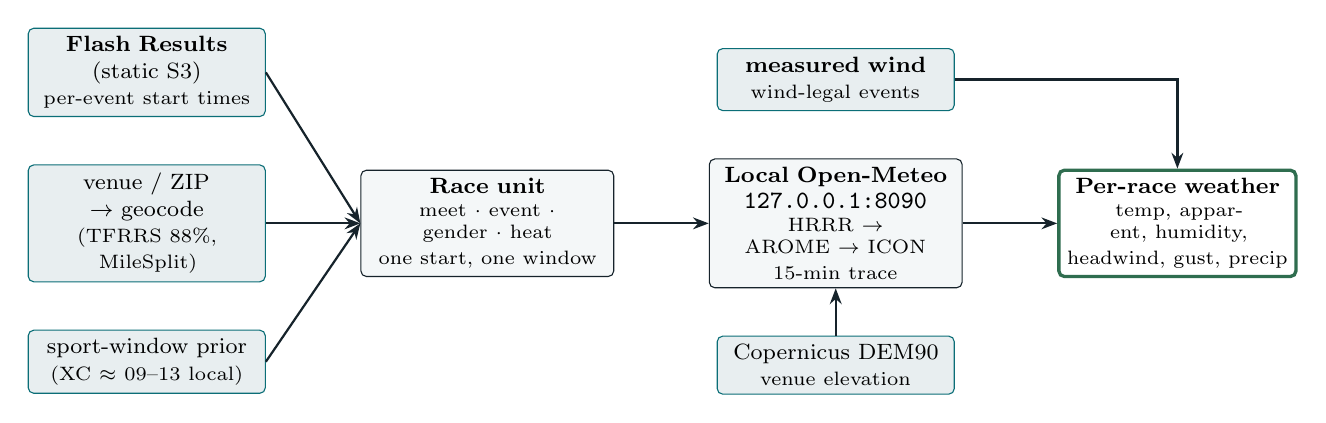
\begin{tikzpicture}[
  font=\footnotesize,
  inp/.style={draw=kailoaccent,fill=kailosoft,rounded corners=2pt,align=center,
             inner sep=3pt,minimum height=7mm,text width=28mm},
  proc/.style={draw=kailoink,fill=boxbg,rounded corners=2pt,align=center,
               inner sep=3pt,minimum height=7mm,text width=30mm},
  res/.style={draw=kailogood,fill=white,rounded corners=2pt,align=center,
              inner sep=3pt,minimum height=7mm,very thick,text width=28mm},
  arr/.style={-{Stealth[length=2mm]},kailoink,thick}
]
% column 1: the three inputs to the race unit
\node[inp] (flash)
  {\textbf{Flash Results} (static S3)\\ \scriptsize per-event start times};
\node[inp,below=6mm of flash] (venue)
  {venue / ZIP $\to$ geocode\\ \scriptsize(TFRRS 88\%, MileSplit)};
\node[inp,below=6mm of venue] (prior)
  {sport-window prior\\ \scriptsize(XC $\approx$ 09--13 local)};

% column 2: the race unit
\node[proc,right=12mm of venue] (race)
  {\textbf{Race unit}\\ \scriptsize meet $\cdot$ event $\cdot$ gender $\cdot$ heat\\
   \scriptsize one start, one window};

% column 3: weather engine + dem
\node[proc,right=12mm of race] (omet)
  {\textbf{Local Open-Meteo}\\ \code{127.0.0.1:8090}\\
   \scriptsize HRRR $\to$ AROME $\to$ ICON\\ \scriptsize 15-min trace};
\node[inp,below=6mm of omet] (dem)
  {Copernicus DEM90\\ \scriptsize venue elevation};
\node[inp,above=6mm of omet] (wind)
  {\textbf{measured wind}\\ \scriptsize wind-legal events};

% column 4: output
\node[res,right=12mm of omet] (wx)
  {\textbf{Per-race weather}\\ \scriptsize temp, apparent, humidity,\\
   \scriptsize headwind, gust, precip};

\draw[arr] (flash.east) -- (race.west);
\draw[arr] (venue) -- (race);
\draw[arr] (prior.east) -- (race.west);
\draw[arr] (race) -- (omet);
\draw[arr] (dem) -- (omet);
\draw[arr] (omet) -- (wx);
\draw[arr] (wind.east) -| (wx.north);
\end{tikzpicture}
\caption{Weather + elevation per \emph{race}, not per meet. The 11\,am women's
JV and the 3\,pm men's varsity get different windows. Wind for sprints comes
measured from the results themselves.}
\end{figure}

\noindent\textbf{Wind is an essential characteristic of a sprint mark.} A 10.90
at $+3.0$ and a 10.90 at $-1.0$ are different performances, and the rule
book agrees (marks over $+2.0$\,m/s are not record-legal). For the wind-legal
events --- 100, 200, the hurdles, long and triple jump --- the measured
gauge reading is stored on the result row itself (Athletic.net carries it on
$\sim$9\% of track rows; TFRRS event pages carry a WIND column), and every
sprint analytic is conditioned on it. Forecast wind from the weather model is
the fallback for distance events, never a substitute for the gauge on a
sprint.

\noindent\textbf{Hill / course difficulty} (three complementary signals):
\begin{enumerate}
  \item \textbf{Empirical ALS course offsets (built).} A two-way log-time model
    --- \(\log(\mathrm{equiv5k}) = \mathrm{ability} + \mathrm{offset}\), i.e.\ an
    athlete-season term plus a course term. \textbf{ALS} is \emph{alternating
    least squares}: hold the course offsets fixed and solve each athlete's
    ability as the least-squares (mean) fit to their races; then hold
    abilities fixed and solve each course's offset the same way; alternate
    until nothing moves (400 rounds), with the offsets anchored to mean zero
    so the split is identified. It needs only athletes who race more than one
    course. Validated split-half \(r=0.98\); recovered Crystal Springs
    $(+72\text{s})$ and Woodbridge $(-50\text{s})$ with no external input. It
    measures what terrain \emph{costs}, but bundles hills with footing and
    weather.
  \item \textbf{External course ratings (cross-check + decomposition).}
    TullyRunners speed ratings, MileSplit course rankings, FloRatings A/B/C/D,
    joshm.dev Crystal Springs Pace Factor, golf-slope analog. Joining these and
    correlating with the ALS offset validates our number and separates
    terrain-driven from conditions-driven difficulty.
  \item \textbf{True elevation gain (targeted).} GPS/GPX course traces through
    the DEM give cumulative climb per km --- the only physical hill metric, but
    per-course external data. Reserve for marquee courses.
\end{enumerate}
\paragraph{Held-out test on 100 athletes per division.} To check that the
offsets carry information rather than fit noise, 100 athlete-seasons with at
least three XC races were drawn at random from each of D1, D2 and D3 (seed
42), one race per athlete was held out, and the model was re-fit on the
remaining 619,056 rows (151,239 athlete-seasons, 3,410 meets). For each
held-out race the question is whether the \emph{course offset} explains what
the athlete's own baseline cannot (Figure~\ref{fig:alsval},
Table~\ref{tab:alsval}): the correlation between the athlete's deviation
from baseline and the course's offset is 0.50--0.76, the prediction error
falls 20--36\% once the offset is applied, and a permutation null (offsets
shuffled across the held-out races, 2,000 draws) never reaches the observed
correlation ($p<0.0005$, null s.d.\ 0.10). D2 is the weakest, consistent
with its thinner meet overlap.

\begin{figure}[H]
\centering
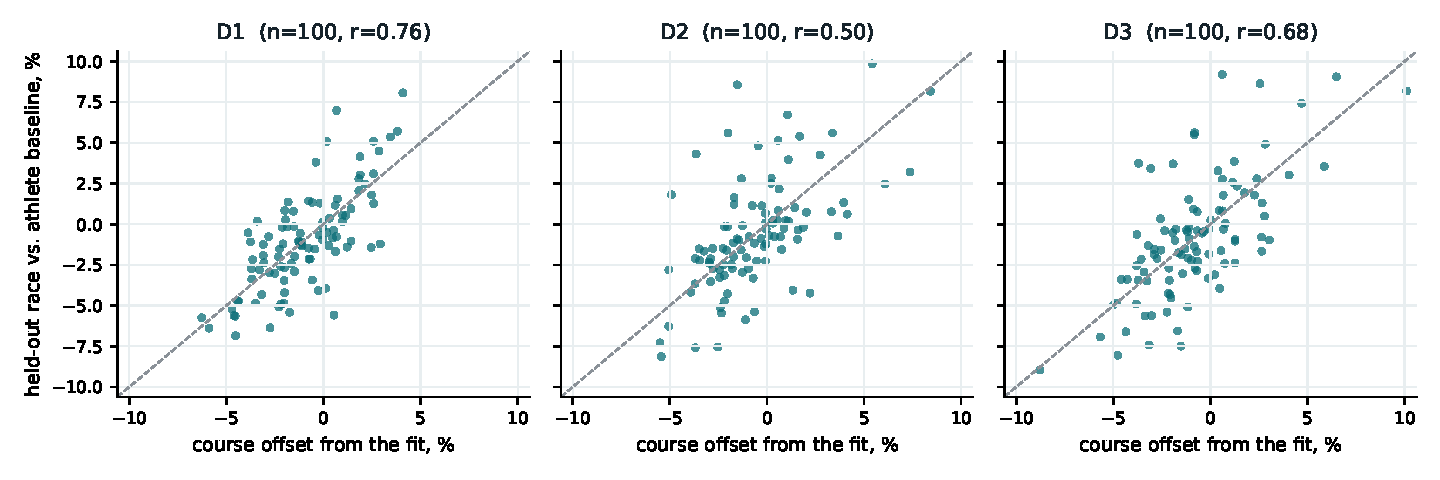
\includegraphics[width=\linewidth]{fig/als_validation.pdf}
\caption{Held-out race vs.\ course offset, 100 random athletes per division.
Each point is one held-out race: $x$ is the course's fitted offset, $y$ is
how far the athlete ran from their own baseline that day. Points on the
dashed line are fully explained by the course.}
\label{fig:alsval}
\end{figure}

\begin{table}[H]
\centering\footnotesize
\begin{tabular}{@{}lrrrrrr@{}}
\toprule
 & $n$ & $r$(dev., offset) & $r$ pred. & $r$ base & MAE base & MAE w/ offset\\
\midrule
D1 & 100 & 0.76 & 0.98 & 0.95 & 28.4\,s & 18.2\,s ($-36\%$)\\
D2 & 100 & 0.50 & 0.97 & 0.97 & 35.4\,s & 28.3\,s ($-20\%$)\\
D3 & 100 & 0.68 & 0.98 & 0.97 & 35.3\,s & 24.1\,s ($-32\%$)\\
\bottomrule
\end{tabular}
\caption{Held-out validation of the ALS course offsets. MAE is on the
5k-equivalent time. Permutation $p<0.0005$ in every division.}
\label{tab:alsval}
\end{table}

Two caveats found while running it. The fit was made on the corpus as it
stands, which still holds 2,705 duplicate XC rows across 46 meets from the
July legacy sync (607 with a conflicting distance label) --- small, and a
targeted delete, but one affected meet's offset is wrong until it is done.
And 259k XC rows belong to schools whose TFRRS slug did not resolve to a
division; the samples are drawn from the 405k that did.

\assess{Once weather is attached per race, re-fit the ALS \emph{net of the
weather term}: the course offset then stops absorbing that day's heat and
becomes a terrain-only score --- the cleanest hill metric derivable without a
GPS trace.}

% ------------------------------------------------------------ DIAGRAM 3 ---
\subsection{(3) Linking college and high-school runners}

There is no crosswalk: zero athletes carry both an Athletic.net id and a TFRRS id, and MileSplit's \code{tfrrsId} field is null on every bio examined. Linkage is therefore \emph{probabilistic}, and the honest deliverable is the ceiling.

\begin{figure}[H]
\centering
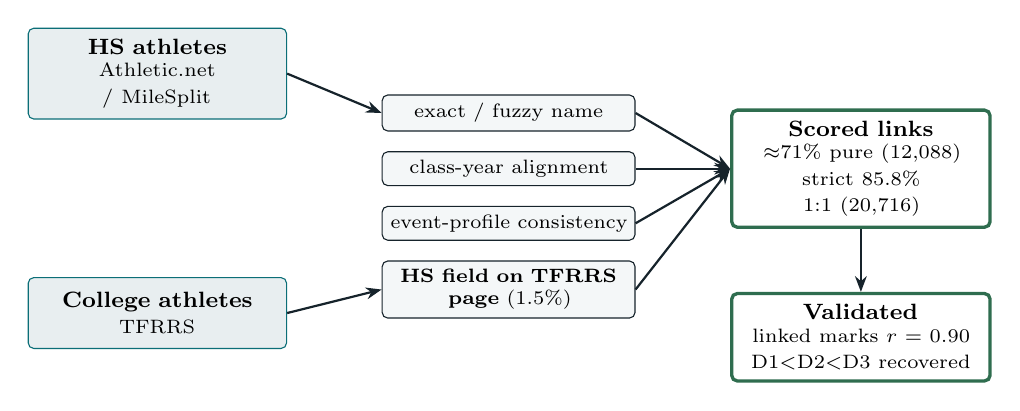
\begin{tikzpicture}[
  font=\footnotesize,
  node distance=6mm,
  pool/.style={draw=kailoaccent,fill=kailosoft,rounded corners=2pt,align=center,
               inner sep=4pt,minimum height=9mm},
  feat/.style={draw=kailoink,fill=boxbg,rounded corners=2pt,align=center,
               inner sep=3pt,font=\scriptsize},
  res/.style={draw=kailogood,fill=white,rounded corners=2pt,align=center,
              inner sep=4pt,minimum height=9mm,very thick},
  arr/.style={-{Stealth[length=2mm]},kailoink,thick}
]
\node[pool,text width=30mm] (hs) {\textbf{HS athletes}\\ \scriptsize Athletic.net\\ \scriptsize / MileSplit};
\node[pool,below=20mm of hs,text width=30mm] (col) {\textbf{College athletes}\\ \scriptsize TFRRS};

\node[feat,text width=30mm,right=12mm of hs,yshift=-5mm] (f1) {exact / fuzzy name};
\node[feat,text width=30mm,below=2.5mm of f1] (f2) {class-year alignment};
\node[feat,text width=30mm,below=2.5mm of f2] (f3) {event-profile consistency};
\node[feat,text width=30mm,below=2.5mm of f3] (f4) {\textbf{HS field on TFRRS page} (1.5\%)};

\node[res,right=12mm of f2,text width=30mm] (link)
  {\textbf{Scored links}\\
   \scriptsize $\approx$71\% pure (12{,}088)\\
   \scriptsize strict 85.8\% 1:1 (20{,}716)};

\node[res,below=8mm of link,text width=30mm] (val)
  {\textbf{Validated}\\ \scriptsize linked marks $r=0.90$\\
   \scriptsize D1$<$D2$<$D3 recovered};

\draw[arr] (hs.east) -- (f1.west);
\draw[arr] (col.east) -- (f4.west);
\draw[arr] (f1.east) -- (link.west);
\draw[arr] (f2.east) -- (link.west);
\draw[arr] (f3.east) -- (link.west);
\draw[arr] (f4.east) -- (link.west);
\draw[arr] (link) -- (val);
\end{tikzpicture}
\caption{Probabilistic HS$\to$college linkage. No exact key exists; a scored combination of name, year and event profile reaches $\sim$71\% precision, and TFRRS athlete pages carry a literal High School field (1.5\% of pages) that opens a path to a \emph{real} crosswalk by crawling those pages directly.}
\end{figure}

\medskip
\noindent\textbf{Why link at all.} The link is what turns two separate
result histories into a \emph{trajectory}. With it the platform can say how
athletes with a given high-school profile developed in college --- expected
first-year 8K from a 3-mile PR, typical improvement by event and by
division, who bloomed late --- and place any current athlete against that
population: Billy Allen's 16:47 3-mile became a 29:39 8K as a freshman, and
the linked population says whether that is ahead of, on, or behind the
curve. That \textbf{potential-growth} view is the core of recruiting (v2):
a prospect's verified HS marks projected forward, rather than a self-reported
PR read at face value. It also benchmarks a program (what HS profile did our
athletes who succeeded arrive with) and lets course-adjusted HS and college
marks be compared on one scale.

\noindent\textbf{The route to a real crosswalk.} TFRRS athlete pages carry a
literal \emph{``High School:''} field on 1.5\% of archived pages (roster pages do
not). Crawling athlete pages directly --- rather than inferring identity from
names --- upgrades the linkage from probabilistic to keyed for the athletes who
have it, and is the recommended next step for the recruiting and progression
models.

\subsection{(4) Finding meets to enter}

A coach's recurring question --- what is coming up, and when do entries
close --- has a scalable answer for high school and an open one for college.

\begin{itemize}
  \item \textbf{High school: MileSplit's meet feed.} The meets endpoint,
    \code{/api/v1/meets} with a \code{state} parameter,
    returns a rolling window of roughly 60 days per state with \code{dateStart},
    \code{dateEnd}, \code{season}, venue city/state and a
    \code{registrationActive} flag (probed 2026-08-22: 100 Indiana meets,
    65 with registration open). It has no deadline field and ignores
    \code{page}, so the pattern is: poll each state once a day (51 requests),
    diff against what was seen, and fetch the meet's own page once for any
    \emph{new} meet with registration open to read the entry deadline. Filter
    by distance from the team's geocode, by level, and by season, and the
    result is an ``upcoming meets near you, entries due by'' list that costs
    a few hundred requests a day nationally.
  \item \textbf{College: the team's own schedule page.} TFRRS lists only past
    meets, and DirectAthletics --- where college entries actually happen ---
    answered our client with a CloudFront 403. But college athletics sites run
    on a handful of templates (Sidearm, PrestoSports), and Rose-Hulman's
    served us without challenge: the schedule page carries every scheduled
    meet with date, host and an \code{.ics} export. Reading a team's schedule
    from its athletics site is uniform across the template and is the
    college route; entry deadlines still come from the coach's DirectAthletics
    account or the host's meet page.
\end{itemize}

\subsection{Build order}
Steps that cost nothing against any host come first:
\begin{enumerate}
  \item Venue + geo columns; reparse venue from the archived TFRRS/MileSplit
    payloads. \textbf{Zero requests.}
  \item Wind column on performances; backfill from archived Athletic.net
    payloads (wind-legal events). \textbf{Zero requests.}
  \item Flash Results time crawler --- new host, static S3, its own polite
    profile and ledger. Start with the NCAA championship/regional set and
    measure the match rate before scaling.
  \item Weather adapter: emit a per-race manifest, run the existing
    \code{\char`\~/weather} Open-Meteo pipeline unchanged, reduce to
    race-window aggregates.
  \item Course difficulty: ship the ALS offset, join external ratings as a
    check, then re-fit net of weather for a terrain-only score.
\end{enumerate}

\subsection{v2 --- Recruiting: considerations and goals}

Recruiting is deliberately a v2 product: it needs the linkage and the
trajectory models above to be real before it is more than a contact list.
Goals, in order:

\begin{enumerate}
  \item \textbf{Prospect lookup with verified marks.} A name resolves to the
    athlete's MileSplit / Athletic.net record, and the page shows their marks
    as the platform holds them --- course-adjusted, wind-conditioned where it
    applies --- not as reported.
  \item \textbf{Potential growth.} The HS $\to$ college trajectory placed
    against the linked population: expected first-year marks, the range, and
    the comparable athletes it is drawn from, by division.
  \item \textbf{Fit to program.} Where the prospect would sit on this roster
    (varsity / JV line, pod) and against the conference, using the same
    projections as the Team tab.
  \item \textbf{Watch lists and timelines.} Prospects by class year with
    contact-period dates, the recruiting file that today lives in the athlete
    person file, and notes.
  \item \textbf{Recruit-visit mode} stays in v1 under Settings: masking
    athlete names on a campus visit is a display toggle, not a recruiting
    feature.
\end{enumerate}

Considerations: NCAA contact rules vary by division and must be encoded, not
assumed; high-school data comes from sources with redistribution terms
(MileSplit's non-commercial etiquette, Athletic.net's ToS), so a commercial
recruiting product likely needs a licensing conversation before it ships; and the
linkage is probabilistic ($\sim$71\% pure today), so every projection must
carry its confidence and its comparables, never a bare number.


\end{document}
